\begin{figure}[H]
    \centering
    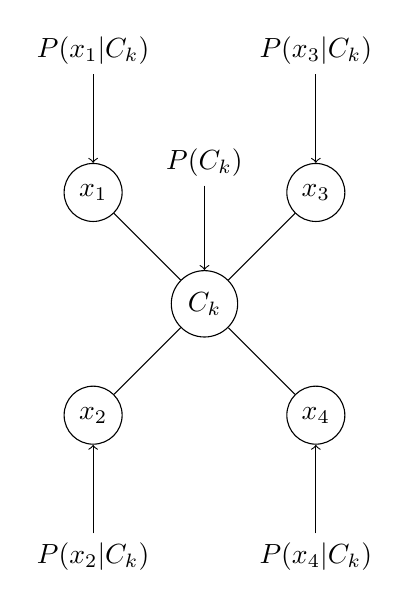
\begin{tikzpicture}[node distance=2cm, auto]
        % Define os nós
        \node[draw, circle] (C) {$C_k$};
        \node[draw, circle, above left of=C] (X1) {$x_1$};
        \node[draw, circle, below left of=C] (X2) {$x_2$};
        \node[draw, circle, above right of=C] (X3) {$x_3$};
        \node[draw, circle, below right of=C] (X4) {$x_4$};
        % Conecta os nós
        \draw[-] (X1) -- (C);
        \draw[-] (X2) -- (C);
        \draw[-] (X3) -- (C);
        \draw[-] (X4) -- (C);
        % Adiciona as probabilidades condicionais
        \node[above of=X1, yshift=-0.2cm] (px1ck) {$P(x_1|C_k)$};
        \node[below of=X2, yshift=0.2cm] (px2ck) {$P(x_2|C_k)$};
        \node[above of=X3, yshift=-0.2cm] (px3ck) {$P(x_3|C_k)$};
        \node[below of=X4, yshift=0.2cm] (px4ck) {$P(x_4|C_k)$};
        % Adiciona as probabilidades a priori
        \node[above of=C, yshift=-0.2cm] (pck) {$P(C_k)$};
        % Adiciona as setas com as fórmulas
        \draw[->] (pck) -- (C);
        \draw[->] (px1ck) -- (X1);
        \draw[->] (px2ck) -- (X2);
        \draw[->] (px3ck) -- (X3);
        \draw[->] (px4ck) -- (X4);
    \end{tikzpicture}
    \caption{Esquema de funcionamento da classifica��o Naive Bayes}
    \label{plt:bayes}
\end{figure}